\input sys/inputs.tex

\usepackage[utf8]{inputenc}
\usepackage[T1]{fontenc}
\usepackage[polish]{babel}
\usepackage{polski}

\begin{document}

\bigheading{Critical Projects}

% \info{task_name}{infile}{outfile}{points}{timelimit}{memlimit}
% leave this values, if you are not interested
\info{critical}{stdin}{stdout}{100}{600 ms}{32 MiB}

Pewien duży projekt został podzielony na $N$ różnych podprojektów.
Kierownik projektu ustalił pewne relacje pomiędzy nimi, mówiące, że pewien podprojekt $u$
	musi zostać całkowicie wykonany przed rozpoczęciem innego podprojektu $v$.
W takiej sytuacji mówimy, że $u$ bezpośrednio poprzedza $v$.
Mówimy, że $u$ poprzedza $v$, jeśli $u$ bezpośrednio poprzedza $v$, albo istnieje podprojekt $z$ taki,
	że $u$ poprzedza $z$ i $z$ poprzedza $v$.

Podprojekt $u$ nazywamy krytycznym, jeśli dla każdego projektu $v$ (różnego od $u$),
	albo $u$ poprzedza $v$, albo $v$ poprzedza $u$.

Wiadomo, że cały projekt można wykonać, czyli nie istnieje podprojekt $u$ taki, że $u$ poprzedza $u$.

\heading{Task}

Napisz program, który znajdzie wszystkie krytyczne podprojekty.

\heading{Input}

W pierwszej linii wejścia znajdują się dwie liczby $N$ i $M$ ($1 \le N \le 100\,000$, $0 \le M \le 1\,000\,000$),
	oznaczające liczbę podprojektów i liczbę znanych relacji poprzedzania.
Podprojekty są ponumerowane liczbami od $1$ do $N$.
Każda z następnych $M$ linii zawiera dwie liczby całkowite $u$ i $v$ ($1 \le u, v \le N$, $u \neq v$),
	oznaczające że podprojekt $u$ bezpośrednio poprzedza podprojekt $v$.

W $40\%$ testów zachodzą dodatkowe warunki: $N \le 5000$ i $M \le 30\,000$.

\heading{Output}

W pierwszej linii wyjścia należy wypisać liczbę krytycznych podprojektów.
W drugiej linii należy wypisać numery krytycznych podprojektów w kolejności rosnącej.
Liczby powinny być oddzielone pojedynczą spacją.
Jeśli nie istnieje żaden krytyczny podprojekt należy wypisać tylko jedną liczbę $0$.

\heading{Sample}

\sampleIN
7 9
1 3
2 3
3 4
3 5
4 6
5 6
1 7
3 7
7 4
\sampleOUT
2
3 6
\sampleCOMMENT

\sampleEND

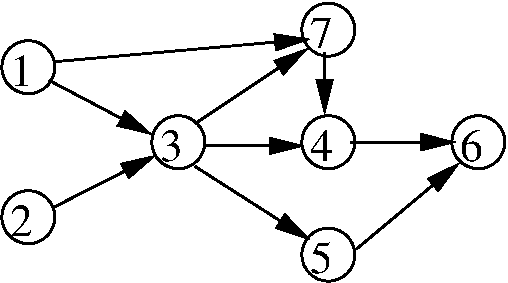
\includegraphics[height=4cm]{img/critical-fig.pdf}
\bigskip

\end{document}
